\documentclass{egpubl}
\usepackage{ceig08}

%\usepackage[ascii]{inputenc}
\usepackage[activeacute,spanish]{babel}
%\usepackage[T1]{fontenc}
\usepackage{amsmath,amssymb,amsfonts,textcomp}
%\usepackage{latexsym}





	% --- for  Annual CONFERENCE
	% \ConferenceSubmission % uncomment for Conference submission
	% \ConferencePaper      % uncomment for (final) Conference Paper
	% \STAR                 % uncomment for STAR contribution
	% \Tutorial             % uncomment for Tutorial contribution
	% \ShortPresentation    % uncomment for (final) Short Conference Presentation
	%
	% --- for  EG Workshop Proceedings
	% \WsSubmission    % uncomment for submission to EG Workshop
\WsPaper         % uncomment for final version of EG Workshop contribution
	%
\electronicVersion % can be used both for the printed and electronic version

	% !! *please* don't change anything above
	% !! unless you REALLY know what you are doing
	% ------------------------------------------------------------------------

	% for including postscript figures
	% mind: package option 'draft' will replace PS figure by a filname within a frame
\ifpdf \usepackage[pdftex]{graphicx} \pdfcompresslevel=9
\else \usepackage[dvips]{graphicx} \fi

\PrintedOrElectronic

% prepare for electronic version of your document
\usepackage{t1enc,dfadobe}

\usepackage{egweblnk}
\usepackage{cite}

% For backwards compatibility to old LaTeX type font selection.
% Uncomment if your document adheres to LaTeX2e recommendations.
\let\rm=\rmfamily    \let\sf=\sffamily    \let\tt=\ttfamily
\let\it=\itshape     \let\sl=\slshape     \let\sc=\scshape
\let\bf=\bfseries

% end of prologue



% ---------------------------------------------------------------------
% ---------------------------------------------------------------------
% ---------------------------------------------------------------------
% ---------------------------------------------------------------------


\begin{document}

\title[Hacia un modelo integral para la generaci\'on de Mundos Virtuales]%
      {Hacia un modelo integral para la generaci\'on\\de Mundos Virtuales}

\author[G. L\'opez, R. Molina \& A. J. Gallego]
       {Gabriel L\'opez Garc\'ia, Rafael Molina Carmona y Antonio Javier Gallego
       S\'anchez\\
       Grupo de Inform\'atica Industrial e Inteligencia Artificial\\
        Universidad de Alicante, Ap.99, E-03080, Alicante, Spain\\
        \{glopez, rmolina, ajgallego\}@dccia.ua.es}



\maketitle


\begin{abstract}
Uno de los problemas m\'as importantes en los sistemas de Realidad
Virtual es la diversidad de los dispositivos visuales y de
interacci\'on que existen en la actualidad. Junto a esto, la
heterogeneidad de los motores gr\'aficos, los motores f\'isicos y los
m\'odulos de Inteligencia Artificial, propicia que no exista un modelo
que a\'une todos estos aspectos de una forma integral y coherente. Con
el objetivo de unificar toda esta diversidad, presentamos un modelo
formal que afronta de forma integral el problema de la diversidad en
los sistemas de RV, as\'i como la definici\'on de los m\'odulos
principales que los constituyen. 

El modelo propuesto se basa en la definici\'on de una gram\'atica, que
integra la actividad necesaria en un sistema de RV, su visualizaci\'on
y su interacci\'on con el usuario. La
descripci\'on de un mundo se presenta como una secuencia ordenada de
primitivas, transformaciones que modifican el comportamiento de las
primitivas y actores que definen la actividad del sistema. Los
conceptos de primitiva, transformaci\'on y actor son mucho m\'as
amplios de lo que es habitual en estos sistemas: Las primitivas no son
simples primitivas de dibujo sino acciones que se deben ejecutar en un
determinado sistema de presentaci\'on, gr\'afico o no; las
transformaciones modifican las primitivas, dependiendo de su
naturaleza; los actores desarrollan una o varias actividades en el
mundo virtual, se visualizan mediante primitivas y transformaciones, y
usan eventos que tambi\'en se definen en sentido amplio.

El modelo presentado tiene como virtud la separaci\'on de la actividad
del sistema de los dispositivos visuales y de interacci\'on concretos
que lo componen. Esto supone varias ventajas: los dispositivos pueden
ser sustituidos por otros dispositivos o por simulaciones de estos, los
elementos del sistema pueden ser reutilizados, y la representaci\'on
gr\'afica puede ser diferente dependiendo del dispositivo visual.
En definitiva, se ha pretendido dise\~nar un
sistema integral, adaptativo, reutilizable y gen\'erico.

Por \'ultimo se presenta un caso pr\'actico que permite concretar c\'omo
se utiliza el modelo propuesto.

\end{abstract}




%___________________________________________________________________________
\section{Introducci\'on
\label{sec:introduccion}}
%___________________________________________________________________________

El desarrollo en las \'ultimas d\'ecadas de los sistemas de Realidad
Virtual (RV) y de los sistemas gr\'aficos en general ha sido
espectacular. Este progreso ha contribuido a que la informaci\'on de
nuestro alrededor se presente mediante gr\'aficas, animaciones o
simulaciones, dando a conocer nuevas formas de an\'alisis. Los
videojuegos constituyen hoy en d\'ia una de las industrias m\'as
pujantes y cada d\'ia nuevos desarrollos de Realidad Virtual aparecen a
nuestro alrededor. Sin embargo, esto no significa que todo est\'e hecho
ni mucho menos, sino que la situaci\'on actual hace que los retos que
se presentan sean a\'un m\'as estimulantes.

 Uno de los problemas m\'as acuciantes es la diversidad de los
dispositivos visuales. Se tiene toda una variedad de dispositivos hardware que
generan im\'agenes (monitores, tel\'efonos m\'oviles, PDAs, gafas de
realidad virtual) y la visualizaci\'on debe adaptarse a cada uno de
ellos seg\'un sus caracter\'isticas particulares (resoluci\'on,
tama\~no, etc.).

 Mientras que todo lo referente a la visualizaci\'on ha alcanzado una
cierta madurez en las pasadas d\'ecadas, en el campo de la
interacci\'on no se ha producido la evoluci\'on deseada \cite{Joshua2004,David2005}. Sigue
dominando el teclado y el rat\'on en los interfaces de usuario, los
mandos con libertad de movimiento son complejos de manejar, y otras
posibilidades de interacci\'on se quedan en el mundo de la
investigaci\'on y el arte gr\'afico \cite{Joshua2004}. Si que es cierto, que en los
\'ultimos a\~nos ha habido t\'imidos avances. Entre ellos se puede
destacar el mando de la Wii.

 Es necesario el desarrollo de alg\'un tipo de modelo que unifique de
alguna forma toda la diversidad de dispositivos para la interacci\'on y
la visualizaci\'on. Por ejemplo, si se desea mover un objeto, ser\'ia
interesante que la acci\'on no se corresponda con una pulsaci\'on de
rat\'on o un determinado bot\'on de un mando, sino que toda esta
diversidad de eventos se unifique en una sola acci\'on, mover el
objeto, y filtre todos los detalles concretos de los dispositivos de
entrada.

 En el desarrollo de un sistema de RV existen tres m\'odulos importantes
que han tenido desigual evoluci\'on. Estos tres m\'odulos son: Motor
Gr\'afico, Motor F\'isico e Inteligencia Artificial. El primero se hace
cargo de todo lo referente a la visualizaci\'on de los datos en
dispositivos visuales, el segundo tiene como objetivo simular todos los
aspectos f\'isicos que hacen que la acci\'on que se desarrolla en la
escena sea coherente y el tercero busca que los actores de la escena se
comporten de una forma independiente mostrando en el mundo virtual
capacidades inteligentes.

 Las diferentes herramientas aportadas en la actualidad para el
desarrollo de los tres m\'odulos anteriores son muy variadas. Existen
m\'ultiples soluciones a diferentes problemas. Sin embargo,
generalmente no se observa ninguna unificaci\'on de criterios a la hora
de abordar los diferentes retos que tiene su desarrollo. Si que es
cierto, por otra parte, que se vislumbran ciertos puntos en com\'un a
la hora de definir determinados dise\~nos estructurales, aunque no se
aprecia un estudio de c\'omo los tres m\'odulos se relacionan entre
s\'i.

 En los pr\'oximos cap\'itulos se presentar\'a un modelo integral que
unifica de forma sencilla y flexible la diversidad que existe en los
sistemas de RV y en los tres m\'odulos anteriormente descritos. Para
ello se utilizar\'a la definici\'on de un lenguaje que integra la
actividad necesaria, su visualizaci\'on y su interacci\'on con el
usuario. En el apartado \ref{sec:antecedentes} se presentan algunos antecedentes de sistemas
de RV. Los objetivos que pretendemos alcanzar centran el contenido del
apartado \ref{sec:objetivos}. En el apartado \ref{sec:modelo} se define el modelo propuesto,
mientras que el \ref{sec:caso_practico} presenta un caso pr\'actico. Por \'ultimo, las
conclusiones y los trabajos futuros se exponen en el apartado \ref{sec:conclusiones}.



%___________________________________________________________________________
\section{Antecedentes
\label{sec:antecedentes}}
%___________________________________________________________________________

Un sistema de RV est\'a formado por tres grandes m\'odulos: 
un motor gr\'afico, un motor f\'isico y un m\'odulo de inteligencia artificial. 
A continuaci\'on se hace un breve repaso de los antecedentes referidos a estos
m\'odulos.

En el desarrollo de los componentes que se utilizan para los motores
gr\'aficos existen dos librer\'ias: Direct3D \cite{DirectX} y
OpenGL \cite{OpenGL}. Ambas librer\'ias se definen como una capa entre la aplicaci\'on y la tarjeta gr\'afica.
Han aparecido sistemas que unifican las dos API 
(\textit{Aplication Program Interfaces}) en un \'unico interfaz. Este es el caso de OGRE
\cite{OGRE}, o de VTK \cite{VTK}.

Existen librer\'ias que se utilizan para gestionar el hardware interactivo.
Dos ejemplos son SDL \cite{SDL} y DirectX \cite{DirectX}. En general, tienen las 
mismas caracter\'isticas salvo que SDL es software libre y est\'a implementada 
tanto para Windows, como para Linux, mientras que la segunda no.

Hay una gran variedad de herramientas que implementan
motores f\'isicos  Como ejemplos se tiene Working Model \cite{WModel},
que realizan simulaciones que se utilizan principalmente en el \'area educativa.
Despu\'es existe Newton Game Dynamics \cite{NGDynamics} Adem\'as existe  Physics Abstraction Layer (PAL) \cite{PAL} 
que es una capa abstracta para el desarrollo de MTR siendo Open Dynamics Engine (ODE) \cite{ODE}
una implementaci\'on de parte de las especificaciones de PAL. Dentro del software propietario 
existen otras tantas API, destancando por un lado PhysX \cite{Physx}, cuyo propietario es NVidia y
es utilizado en la PlayStation 3, y Havok \cite{Havok}, perteneciente a
la compa\~n\'ia Havok y que est\'a implementado para Windows, Xbox 360,
Wii, PlayStation3 y PlayStation Portable, Mac OS X y Linux.

Los \'ultimos tipos de herramientas son los que desarrollan el m\'odulo
de IA. No existen librer\'ias que puedan ser utilizadas como soluciones 
gen\'ericas, salvo en alg\'un caso. Su n\'umero es escaso y cada sistema 
de IA est\'a dise\~nado
espec\'ificamente para una aplicaci\'on concreta. Uno de los motivos
por los que los sistemas de IA se han desarrollado con mayor lentitud
que el resto de sistemas podr\'ia ser el esfuerzo que se realiza por
mejorar el aspecto gr\'afico de los juegos, y no tanto por la
inteligencia de sus personajes \cite{Laird2001}. A\'un as\'i, podemos especificar
varios tipos de sistemas: Sistemas evolutivos y Sistemas basados en
agentes.

Dentro de los sistemas evolutivos hay alguna herramienta que facilita
el uso de dichos algoritmos. Podemos destacar EO Evolutionary Computation Framework
\cite{EOECF} desarrollado en C++ y que implementa lo necesario para el
desarrollo de algoritmos evolutivos. Tambi\'en existe CILib
\cite{CILib}, entorno de desarrollo implementado en Java. Por el
contrario, s\'i que se puede encontrar una gran variedad de art\'iculos
que describen el desarrollo de algoritmos gen\'eticos y art\'iculos que
definen sistemas evolutivos para casos concretos \cite{Georgios2004,Chris2007,Robert2005}.

En cuanto a los sistemas basados en agentes, se puede obtener una
extensa literatura que detalla los aspectos de este tipo de elementos,
como por ejemplo en \cite{Wooldridge1997,Wood2000}. En algunos casos, estos agentes se
denominan \textit{bots}, sobre todo en el desarrollo de juegos en
primera persona. Actualmente, este tipo de sistemas est\'an muy
extendidos en grupos de investigaci\'on para el desarrollo de IA, tanto
para juegos como para simulaciones sociales y desarrollo de robots
m\'oviles \cite{John2007,Kenyon2006}. Existen varios entornos que nos simplifican la
tarea para desarrollar \textit{bots}, aunque estos son sistemas para
juegos concretos: por ejemplo se tiene QuakeBot para el juego Quake y
FlexBot para el juego Half-Life \cite{Laird2001,Aaron2002}. Existen librer\'ias m\'as
gen\'ericas para el desarrollo de Agentes, por ejemplo Jade
\cite{Jade}, que modela sistemas multiagentes basados en Java. 



%___________________________________________________________________________
\section{Objetivos
\label{sec:objetivos}}
%___________________________________________________________________________


Los objetivos se orientan principalmente a conseguir un modelo que
integre los diferentes m\'odulos que forman parte de un sistema de RV y
que tenga una total independencia de los dispositivos hardware, tanto
visuales como de interacci\'on, pudiendo, si fuera necesario, sustituir
un dispositivo por otro, o por una simulaci\'on, sin afectar a los
mecanismos internos del sistema. Para lograr esto se pretende:


\begin{enumerate}
	\item Definir un motor gr\'afico que elimine la diversidad de los
	diferentes dispositivos visuales. Es decir, se desea que con una
	\'unica descripci\'on de la escena se procese la misma, de tal manera
	que se muestre en cualquier dispositivo gr\'afico y con un nivel de
	detalle acorde con las caracter\'isticas gr\'aficas del dispositivo.
	
	\item Definir un motor f\'isico que modele toda la actividad del
	sistema, adapt\'andose a los diferentes componentes hardware donde se
	va a ejecutar. Si se dispone de componentes hardware que implementan
	algoritmos f\'isicos, el sistema debe aprovecharlos, pero si por el
	contrario no existen, los debe implementar mediante software.
	
	\item El motor de IA se debe integrar con el motor f\'isico considerando
	las limitaciones impuestas por este. Esto supone que se debe realizar
	un trabajo importante en la integraci\'on de un motor sobre el otro.
	
	\item Se pretende que la interacci\'on con el sistema no dependa del
	hardware de entrada, si no que se abstraiga del origen de la
	interacci\'on, y procese directamente las \'ordenes del usuario.
	
	\item La reutilizaci\'on de los diferentes elementos de forma casi
	inmediata. Si, por ejemplo, se dise\~na un elemento para un determinado
	mundo virtual, utilizando los mecanismos proporcionados por el sistema,
	se podr\'a reutilizar dicho componente en cualquier otro mundo virtual
	o aplicaci\'on que gestione un sistema de RV.
\end{enumerate}


Para la realizaci\'on de todos estos objetivos se utilizar\'an modelos
matem\'aticos que formalizar\'an los diferentes componentes del
sistema, abstrayendo las caracter\'isticas que definen los tres
m\'odulos importantes de un sistema de RV. 


%___________________________________________________________________________
\section{Modelo para la generaci\'on de Mundos Virtuales
\label{sec:modelo}}
%___________________________________________________________________________

Un mundo virtual se caracteriza por un conjunto de actores o elementos,
con una descripci\'on geom\'etrica y que realizan una actividad en un
escenario. La actividad puede o no modificar objetos que componen el
escenario, as\'i como el aspecto del actor o de otros actores.

La descripci\'on de un mundo se puede
considerar como una secuencia ordenada de primitivas, transformaciones
que modifican el comportamiento de las primitivas y actores que definen
la actividad dentro del sistema. El concepto de primitiva se debe
considerar, no como una primitiva de dibujo tal como una esfera, un
cubo, etc. sino m\'as bien como una acci\'on que se debe ejecutar en
un determinado sistema de visualizaci\'on. Por ejemplo, dentro del
concepto de primitiva cabe considerar la ejecuci\'on de un sonido. Los
actores, por su parte, ser\'an los componentes que desarrollen una o
varias actividades en el mundo virtual y que se visualizar\'an mediante
primitivas y transformaciones. Para modelar las diferentes actividades
de los actores se va a usar el concepto de evento, eso s\'i,
considerando un evento, no como una acci\'on generada por un
dispositivo de entrada, sino m\'as bien como una acci\'on que
representa la activaci\'on de una determinada actividad que puede ser 
ejecutada por uno o varios actores.

A cada elemento que compone una
escena se le puede asignar un s\'imbolo, formando un conjunto de
s\'imbolos. Con este conjunto se puede construir diferentes cadenas que
describen una escena. Estas cadenas
deben construirse con una sintaxis
definiendo un lenguaje. Habitualmente una sintaxis se presenta como una
gram\'atica \cite{Davis1994}, en adelante denotada por
M, que queda definida por la tupla $M~=~<~\Sigma,~N,~P,~S~>$. 
Con la gram\'atica $M$ se determinar\'a el lenguaje
$L(M)$. La definici\'on de la tupla gramatical se expresa como:

\begin{itshape}
	Sea P el conjunto de s\'imbolos que define un conjunto de primitivas.
	
	Sea T el conjunto de s\'imbolos que define las transformaciones.
	
	Sea O = \{ {\textperiodcentered} ( ) \} el conjunto de s\'imbolos de
	separadores y operaciones.
	
	Sea D el conjunto de tipos de eventos generados para el sistema.
	
	Sea $A^{D}$ el conjunto de s\'imbolos que representan
	actores que van a activarse para los eventos enumerados en el
	super\'indice. Por ejemplo, el actor $a^{d}$ ser\'a
	ejecutado cuando se produzca un evento $e^{d}$.
	
	Sea $\Sigma = P \cup T \cup O \cup A^{D}$ el
	conjunto de s\'imbolos terminales.
	
	Sea N = \{mundo, variosObjetos, objeto, actor, transformaci\'on,
	figura\} el conjunto de s\'imbolos no terminales.

	Sea S = \{mundo\} el s\'imbolo inicial de la gram\'atica.
\end{itshape}



Definimos las reglas gramaticales P como:


\begin{center}

\begin{tabular}{|l|}
	\hline

	\textbf{mundo} :- variosObjetos \\
	
	\textbf{variosObjetos} :- objeto {\textbar} objeto {\textperiodcentered} variosObjetos\\
	
	\textbf{objeto} :- figura {\textbar} transformaci\'on {\textbar} actor\\
	
	\textbf{actor} :- $a^{d}$(variosObjetos), $a^{d} \in M^{D}, d \in D$\\
	
	\textbf{transformacion} :- $t$(variosObjetos), $t \in T$\\
	
	\textbf{figura} :- $p$, $p \in P$\\

	\hline
\end{tabular}
\end{center}


La gram\'atica $M$ es una gram\'atica independiente del contexto,
o de tipo 2, y por tanto se asegura que existe un
procedimiento que verifica si una escena est\'a bien descrita o no, o
dicho de otro modo, que la cadena pertenece o no al lenguaje $L(M)$. Es
decir, se podr\'a determinar que, por ejemplo, la cadena
$a_{1}^{d} ( p_{1} \cdotp p_{2} ) \cdotp p_{3} \cdotp t_{1} ( p_{1} \cdotp p_{2}) \in L(M)$ 
donde
$p_{i} \in P$, 
$t_{i} \in T$, 
$a_{i}^{d} \in A^{D}, d \in D$,
pero que la cadena
$a_{1}^{d} \cdotp p_{1} \notin L(M)$.


Sin embargo, se necesita saber cu\'al va a ser
la funcionalidad de las diferentes cadenas. Se puede considerar que la
sem\'antica de una lenguaje explica esta funcionalidad. La sem\'antica
tiene varias formas de definici\'on: operacional, denotacional y
axiom\'atica. En el caso presente se va
a utilizar el m\'etodo denotacional que
describe funciones matem\'aticas para cada una de las cadenas.

La sem\'antica del actor se describe como la
ejecuci\'on del mismo cuando recibe o no un evento que debe manejar.
Esta ejecuci\'on se representar\'a como una funci\'on que define la
evoluci\'on del actor a trav\'es del tiempo. Esto significa que va a
cambiar la cadena que describe su actual estado. La funci\'on que
define el comportamiento de un actor para un evento producido se
denomina \textit{funci\'on evolutiva del
actor} y se denotar\'a con $\lambda$. Su expresi\'on viene dada por:

\begin{equation}
 	\lambda (a^{d}(v),e^{f})=
	\left\{
	\begin{array}{ll}
		u \in L(M) & \mathit{Si}  \ \ f = d \\
		a^{d}(v)  & \mathit{Si}  \ \ f \neq d 
	\end{array}\right\}
\end{equation}

El resultado de la funci\'on $\lambda$ puede
contener o no al propio actor o puede generar otro evento para la
siguiente etapa. Si se desea acumular un
evento para la siguiente etapa se utilizar\'a la notaci\'on
$\Delta e^{f}$.
Esto permitir\'a que los actores puedan generar eventos, y pasen a la
siguiente etapa acciones que puedan recoger otros actores implementando
un proceso de retroalimentaci\'on del sistema. En el caso de que el
evento no coincida con el evento activador entonces la funci\'on
devuelve el mismo actor. M\'as adelante se ver\'a que las funciones
$\lambda$ pueden clasificarse seg\'un las cadenas que se definan en
su evoluci\'on. Sobre todo, van a ser esenciales para la
visualizaci\'on del sistemas determinadas funciones $\lambda$, que
solo devuelven cadenas con primitivas y transformaciones.

Con la funci\'on $\lambda$ se puede definir un algoritmo que, dado un
conjunto de eventos y una cadena, describe como el sistema evoluciona.
A esta funci\'on se la llamar\'a funci\'on de evoluci\'on $\alpha$
del sistema. Para su definici\'on se necesita un conjunto de eventos
$e^{i}, e^{j}, e^{k}, ..., e^{n}$ que abreviando se
denotar\'a como $e^{v}$ siendo
$v \in D^{+}$. La funci\'on se define como:

\begin{equation}
	\alpha (w,e^{v}) = \left\{
	\begin{array}{cl}
		w 	& \mathit{Si} \ \ w \in P  \\

		t(\alpha (v,e^{v})) 	& \mathit{Si}  \ \  w = t(v)  \\

		\underset{\forall f \in v}{ \prod }(\lambda (a^{d}(\alpha
			(y,e^{v})),e^{f})) 	& \mathit{Si}  \ \ w = a^{d}(y)  \\

		\alpha (s,e^{v}) \cdot \alpha (t,e^{v}) 	& \mathit{Si}  \ \  w = s \cdot t 
	\end{array}\right\}
\end{equation}


El operador $\underset{\forall f \in v}{\prod }(\lambda (a^{d}(x),e^{v}))$ 
realiza la concatenaci\'on de la cadenas generadas por
$\lambda$. Se debe observar que para las cadenas que
solo son transformaciones y primitivas,
el sistema se queda como est\'a y no
forman parte de su evoluci\'on. Este tipo de cadenas van a ser
importantes a la hora de optimizar el
sistema, ya que solo ejecutaremos
$\alpha$ para aquellas cadenas que sean actores.

Por otro lado, est\'an las primitivas cuya sem\'antica ser\'a definida
mediante la funci\'on $\gamma$. Dado un s\'imbolo del alfabeto $P$
ejecuta una primitiva sobre lo que se denominar\'a una geometr\'ia
aplicada $G$. Por tanto, la funci\'on ser\'a una aplicaci\'on definida
como:

\begin{equation}
	\gamma: P \rightarrow G	
\end{equation}



Esto significa que dependiendo de la funci\'on ${\gamma}$, el resultado
variar\'a seg\'un la definici\'on que se haga de $G$. Esta $G$ se puede
definir como las acciones que se ejecutan en una librer\'ia gr\'afica
concreta, como OpenGL o Direct3D. Se relacionar\'an los s\'imbolos de $P$
con la ejecuci\'on de funciones de la librer\'ia y si, por ejemplo,
$esfera \in P$ se podr\'a ejecutar la funci\'on que dibuja
una esfera en OpenGL o Direct3D:


\[ \begin{matrix}
	\gamma_{opengl}(esfera) = glutSolidSphere \\
	\gamma_{direc3d}(esfera) = drawSphereDirect3D
\end{matrix} \]


Sin embargo, esta definici\'on no solo se puede utilizar para
librer\'ias gr\'aficas, sino que se puede ampliar a otras definiciones.
Por ejemplo, se puede definir para el mismo alfabeto P otra funci\'on
$\gamma_{bounds}$ que calcule los l\'imites de la figura
que define una primitiva. Es decir, si
{\textquotesingle}\textit{boundSphere}{\textquotesingle} es una
funci\'on que implementa el c\'alculo de los l\'imites de una esfera,
entonces:

\[ \gamma_{bounds}(esfera) = boundSphere \]



Los ejemplos anteriores demuestran que la funci\'on $\gamma$ aporta
toda la abstracci\'on necesaria para homogeneizar las diferentes
implementaciones que existen para realizar la definici\'on de un mundo
concreto.


Sin embargo, solo se han tratado elementos geom\'etricos o de dibujo.
No hay ninguna restricci\'on al respecto siempre y cuando exista la
definici\'on para esta primitiva en la funci\'on $\gamma$. As\'i,
tambi\'en se pueden considerar como primitivas la ejecuci\'on de un
sonido, el reflejo de un material, el color de un personaje, el
movimiento de un robot, la manipulaci\'on de una m\'aquina, etc.
Adem\'as, la definici\'on de la funci\'on $\gamma$ tambi\'en describe
sistemas que escriban diferentes formatos de ficheros (VRML, DWG, DXF,
XML, etc.), transporten cadenas por la red, ejecuten instrucciones de
una m\'aquina que realiza esculturas 3D, etc.


Por \'ultimo, la gram\'atica define lo que son las transformaciones que
modifican el comportamiento de las primitivas. Estas transformaciones
tienen un \'ambito de aplicaci\'on y deber\'an ser aplicadas a
determinado conjunto de primitivas. Es decir, se desea que una
transformaci\'on $t \in T$ se aplique sobre una subcadena $w$ que se
simboliza en el lenguaje como $t(w)$. Para definir el \'ambito de
aplicaci\'on de una trasformaci\'on se definen las siguientes funciones
sem\'anticas:

\begin{center}
\begin{tabular}{l}
	I: T ${\rightarrow}$ G (Inicia transformaci\'on) \\

	F: T ${\rightarrow}$ G (Finaliza transformaci\'on)
\end{tabular}
\end{center}


Estas dos funciones tienen las mismas caracter\'isticas que la
funci\'on $\gamma$ pero aplicadas al conjunto de transformaciones
anteriormente descritas.


Existe una restricci\'on sobre las tres \'ultimas funciones, y es que
no pueden ser aplicadas sobre actores. Es decir, no se puede ejecutar
$\gamma(a_{1}^{d}(w))$, ni
$I(a_{1}^{d}(w))$, ni
$F(a_{1}^{d}(w))$. Se debe primero
transformar el actor en una cadena de primitivas y transformaciones,
que ser\'a su representaci\'on gr\'afica. Por ejemplo, si se define
un actor que describe la actividad de una nave espacial, se debe
transformar el actor en una secuencia de primitivas y transformaciones
que van a representar la imagen de la nave espacial.

Como se ha dicho con anterioridad, las funciones $\lambda$ se pueden
clasificar seg\'un la cadena de resultados que devuelvan. Uno de los
tipos de funciones $\lambda$ son aquellas que devuelven solo cadenas
que sean primitivas y transformaciones. A estas funciones se les va a
denominar funci\'on de aspecto $\tau$ y su expresi\'on es:



\begin{equation}
	\tau (a^{d}(v), e^{f}) = \left\{
	\begin{matrix}
		z \in L(E)  & \mathit{Si} \ \ f = d  \\

		\epsilon  & \mathit{Si} \ \ f \neq d  
	\end{matrix}\right\}
\end{equation}


Se puede observar que existen peque\~nas diferencias entre $\lambda$
y $\tau$. La primera es que $\tau$ devuelve cadenas que pertenecen a
$L(E)$, siendo este el lenguaje de la gram\'atica $E$ que es igual que $M$
pero eliminado los actores. Adem\'as si no coincide
con el evento devuelve una cadena vac\'ia. Esto quiere decir que para ese evento
el actor no tiene representaci\'on en la vista. El tipo de evento es
importante y no se corresponde con ning\'un dispositivo de entrada en
concreto, si no m\'as bien es un evento que se encargar\'a de
establecer los diferentes tipos de vista que tiene el sistema. As\'i,
si se desea un sistema de dibujo que filtre determinados elementos para
que queden invisibles, solo tienen que no reaccionar al evento. Estos
eventos tambi\'en sirven para decidir qu\'e tipo de visualizaci\'on se
desea, dependiendo de la ventana o dispositivo de salida.


Al igual que con $\lambda$, se define un algoritmo para
${\tau}$ que dado una cadena $w \in L(M)$ y un conjunto de eventos
$e^{v}$ con $v \in V^{+}$ y $V \subset D$, siendo $V$ los tipos de eventos para
visualizar el sistema, se devuelva una cadena $v \in L(E)$. A
esta funci\'on le denominamos funci\'on de visualizaci\'on $\Omega$ y
se define como:

\begin{equation}
 	\Omega (w, e^{v}) = \left\{
	\begin{matrix}
		w    &    \mathit{Si} \ \ w \in P  \\

		t( \Omega (y, e^{v}))    &    \mathit{Si} \ \ w = t(y)  \\

		\underset{ \forall f \in v} {\prod} \tau (a^{d} (\Omega (y, e^{v})), e^{f})  &
			\mathit{Si}  \ \ w = a^{d}(y)   \\

		\Omega (s, e^{v}) \cdot \Omega (t, e^{v})   &  \mathit{Si} \ \ w = s {\cdot} t
	\end{matrix}\right\}
\end{equation}



Se puede comprobar que es igual que la
funci\'on $\alpha$ salvo que sustituimos $\lambda$ por $\tau$ y que los eventos que
pueden ser pasados a la funci\'on solo pueden pertenecer a $V$. 
En el caso de que a la funci\'on $\Omega$ se le pase
un evento que no pertenece a $V$ lo \'unico que producir\'a ser\'a una
cadena vac\'ia.





%___________________________________________________________________________
\subsection{Actividad y Eventos
\label{sec:actividad_eventos}}

La actividad en un sistema de RV la representan los actores. Esta
actividad suele realizarse entre actores del propio sistema y entre 
dispositivos de entrada y cadenas de la escena.

Toda actividad consiste en un proceso que se produce en un sistema como
reacci\'on a un determinado evento. Este evento puede ser producido por
otra actividad o por un dispositivo de entrada. Como resultado de una
actividad se puede producir una modificaci\'on de los estados de los
actores que forman el sistema. As\'i, se puede ver que lo que define a
una actividad es, por un lado, el proceso de ejecuci\'on de la
actividad que realiza el actor, y por otro, el evento o el conjunto de
eventos que van a activar dicha actividad.

El concepto de evento dentro de un actor es importante, ya que define
cu\'ando se va a ejecutar la actividad independientemente del origen
del evento. Esta independencia es necesaria para la generalizaci\'on de
los dispositivos de entrada, ya que independiza el dispositivo de la
actividad que se debe procesar.

La generalizaci\'on de los eventos facilita la realizaci\'on de
simulaciones. Por ejemplo, si se quiere hacer una simulaci\'on en la
que un usuario mueve un determinado elemento, solo se deben generar
tantos eventos de {\textquotesingle}movimiento{\textquotesingle} como
se desee, simulando la presencia del usuario. Tambi\'en, se puede
simular la existencia de dispositivos. Por ejemplo, simular la
existencia de un guante de realidad virtual con un rat\'on. Para ello,
se debe generar aquellos eventos producidos por el guante de realidad
virtual.

Ya se ha visto que la identificaci\'on del evento es uno de los
atributos dentro de la actividad de un sistema de RV. Pero adem\'as, en
un evento se pueden definir unos datos que caracterizan a una instancia
del evento. Por ejemplo, un evento de movimiento puede contener los
datos del movimiento. Por supuesto, pueden existir eventos que no
tengan datos asociados.

No toda actividad tiene porqu\'e ejecutarse cuando se env\'ia un evento.
Pueden existir determinados eventos que ejecutan la actividad si se
cumplen ciertas condiciones, dependiendo del estado del actor. Esta
comprobaci\'on va a estar definida en el evento y no en el objeto que
tiene definida la actividad. Por tanto, se va a establecer una
definici\'on de evento:


\begin{itshape}
	Se define $e_{c}^{d}$ como el evento de tipo
	{\textquotesingle}d{\textquotesingle}, que tiene como datos
	{\textquotesingle}e{\textquotesingle} y que se ejecuta de forma
	opcional bajo la condici\'on {\textquotesingle}c{\textquotesingle}.
\end{itshape}


Se puede observar que el origen de la creaci\'on de dichos eventos
puede ser cualquiera, y que no es importante el origen, sino m\'as bien
el tipo de evento que se quiere enviar y su definici\'on.



%___________________________________________________________________________
\subsection{Dispositivos de entrada
\label{sec:dispositivos_entrada}}


Se desea establecer una independencia entre el sistema y los
dispositivos de entrada. Por tanto, se necesita definir, para un
conjunto de dispositivos de entrada, los eventos necesarios para hacer
reaccionar al sistema. Por ejemplo, si tenemos un rat\'on y se quiere
mover un personaje de un juego, no se tiene que definir para el
personaje el evento de rat\'on, sino que el rat\'on va a definir un
evento que genera el movimiento del personaje.

Para ello, se va a especificar una funci\'on que, dependiendo del
dispositivo, va a generar los eventos que se necesitan para hacer
reaccionar al sistema. A este elemento se va denominar
\textit{generador de eventos} y su definici\'on es:


{\itshape
Se define como $G^{D}(t)$ al generador que crea los
eventos del tipo $d$ en el instante $t$, siendo $d \in D$ donde $D$ es el
conjunto de tipos de eventos que pueden ser generados.}


En la definici\'on anterior se debe destacar que los eventos se generan
en un instante $t$. Esto se debe a motivos de sincronizaci\'on. Existe
adem\'as la posibilidad de que $G$ no cree ning\'un evento.

Con esta definici\'on se independiza los dispositivos de entrada del
sistema de RV. As\'i, se puede crear un generador para un rat\'on,
para un guante, para un teclado o para cualquier dispositivo de entrada
y que puedan generar los mismos tipos de eventos. Lo interesante de la
implementaci\'on del generador es que solo se tendr\'a en un sitio la
parte dependiente del dispositivo de entrada.

La actual definici\'on de generador de eventos no tiene porqu\'e estar
asociada a un dispositivo de entrada hardware, sino que tambi\'en se
pueden asociar a procesos software. Estos procesos software pueden ser
de cualquier \'indole: de colisi\'on entre elementos, de
contabilizaci\'on, de acumulaci\'on de informaci\'on para que en los
instantes siguientes se produzcan otros eventos, etc. En definitiva,
cualquier proceso que interact\'ue con el sistema.

Existe el problema de que varios generadores pueden crear eventos del
mismo tipo y con distintos datos. Para que esto no cree conflictos se
va a establecer un orden de prioridad entre los distintos generadores,
de forma que, dados dos generadores $G_{i}$ y
$G_{j}$, se creen dos eventos del mismo tipo, por lo que
prevalecer\'a el evento creado por $G_{i}$ sobre el de
$G_{j}$. Por ejemplo, si existe un teclado, un rat\'on y un
\textit{joystick}, se puede establecer el siguiente orden de prioridad:
1{\textordmasculine} \textit{Joystick}, 2{\textordmasculine} Rat\'on,
3{\textordmasculine} Teclado. Estos procesos de redundancia se producen
porque el sistema debe ser implementado para todos estos
dispositivos. Si existen varios, solo prevalecer\'a uno de ellos. El
orden de prioridad se puede establecer, por ejemplo, por orden de
inmersi\'on en el sistema o facilidad de uso. En el caso de que no
exista uno de los dispositivos, actuar\'ia el de siguiente prioridad.

El proceso para la obtenci\'on de los eventos producidos por todos los
dispositivos de entrada y sus generadores asociados se define como:

\begin{itshape}
Se define $G^{*}$ como el conjunto de todos los generadores de
eventos del sistema asociados a los dispositivos de entrada.

Se define $e(z, e^{i})$ siendo $G_{i}(t) = e^{i}$, como:

\[
	e(z, e^{i}) = \left\{
	\begin{matrix}
		z \cdot e^{i}   &   \mathit{si} \ \ e^{i} \notin z \\
		z    &   \mathit{si} \ \ e^{i} \in z
	\end{matrix}
\right\}\]


La funci\'on $E(G^{*},t)$ que recolecta todos los eventos
de todos los generadores se define como:

\[
	E(G^{*}, t) = \left\{
	\begin{matrix}
		e(z, G_{i}(t))   &   z = E(G^{*} - G_{i}, t) \\
		\epsilon   &  \mathit{si} \ \ G^{*} = \emptyset 
	\end{matrix}
\right\}\]


\end{itshape}



%___________________________________________________________________________
\subsection{Algoritmo del sistema
\label{sec:algoritmo_sistema}}

Una vez definidos todos los elementos implicados en el modelo que
gestionar\'a un sistema de RV se puede establecer el algoritmo que
ejecutar\'a todo el sistema, tanto la evoluci\'on como la
visualizaci\'on del mismo, para cada instante $t$ o frame. El
algoritmo es:


\begin{itshape}
Sea D = \{ Conjunto de todos los tipos de eventos posibles en el
sistema\}.

Sea V = \{ Conjunto de todos los tipos de eventos de dibujo\} con
$V \subset D$.


Sea $G^{*}$ = \{ Todos los generadores de eventos que genera eventos de tipo D\}

Sea g el dispostivivo de salida.

Sea $e^{*}$ todos los eventos generados por el sistema.

Sea $e^{v}$ todos los eventos de los dispositivos visuales. Estos eventos ser\'a
una de las entradas de la funci\'on de visualizaci\'on del sistema $\Phi$.

Sea $e^{u}$ todos los dem\'as eventos que no son visuales. Estos eventos ser\'a la entrada de 
la funci\'on de evoluci\'on del sistema $\alpha$.


Se define el algoritmo Generador de Mundos Virtuales como:


Paso 1. Sea $w = w_{o}$ donde $w_{o}$ es la cadena inicial del sistema.


Paso 2. Sea $t = 0$.


Paso 3. $e^{*} = E(G^{*}, t)$


Paso 4. $e^{v} =$ Evento de $e^{*}$ donde $v \in V^{+}$


Paso 5. $e^{u} = e^{*} - e^{v}$


Paso 6. $w_{sig} = \alpha (w, e^{u})$


Paso 7. $v = \Omega (w, e^{v})$


Paso 8.$g=\Phi (v)$


Paso 9. $w = w_{sig}$; $t = t+1$


Paso 10. Si $w = \varepsilon$ entonces ir a Paso 12.


Paso 11. Ir a paso 3.


Paso 12. Fin.

\end{itshape}

\begin{figure}[htb]
  	\centering
	\begin{tabular}{cc}
  		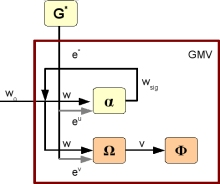
\includegraphics[width=3.5cm]{img/figura3}
	\end{tabular}
 	\caption{\label{fig:ejemplo} Diagrama del Algoritmo Generador de Mundos Virtuales}
\end{figure}

Los dos primeros pasos del algoritmo conforman la parte de la inicializaci\'on del sistema. Esto es, al sistema se le introduce el estado inicial de la escena $w_{o}$ y el primer frame va a ser el 0.

Los pasos 3, 4 y 5 gestionan los eventos del sistema. Primero se llama a los generadores y se asigna a una lista $e^{*}$ todos los eventos generados. En los pasos 4 y 5 se dividen los eventos en eventos para la visualizaci\'on $e^{v}$ y los dem\'as eventos $e^{u}$. La primera ser\'a una de las entradas a la funci\'on $\Omega$ y la segunda a la funci\'on $\alpha$.

En el paso 6, con la cadena actual del sistema $w$ y los eventos que no son de visualizaci\'on ($e^{u}$), se llama a la funci\'on de evoluci\'on $\alpha$ para calcular la cadena del siguiente frame o instante $t$.

En el paso 7 y 8 se realiza la visualizaci\'on del sistema. En primer lugar se transforman los actores en primitivas y transformaciones llamando a la funci\'on $\Omega$ y con los eventos de visualizaci\'on $e^{v}$. Una vez se tiene la cadena que representa la visualizaci\'on del sistema en este instante $t$ se llama a la funci\'on $\Phi(v)$ para visualizar el sistema en el motor gr\'afico.

En el paso 9 se prepara para la siguiente iteraci\'on y se asigna $w$ a $w_{sig}$ y se aumenta en 1 el n\'umero de frames o instantes.

En el paso 10 se mira si se ha llegado a la condici\'on de finalizaci\'on, esto es, si la cadena siguiente es vac\'ia y si es cierto se termina el algoritmo, paso 12. En caso contrario, se vuelve al paso 3 para el siguiente frame.

Se puede destacar que el paso 6 es intercambiable con los pasos 7 y 8 porque no comparten datos que tengan que modificar. Esta caracter\'istica es importante para la implementaci\'on en paralelo del algoritmo. Efectivamente, si este algoritmo se desea paralelizar se puede poner en tareas diferentes el paso 6 por un lado, y los pasos 7 y 8 por otro.

Tambi\'en se puede observar que para que termine el algoritmo solo se debe devolver en $\alpha$ una cadena vac\'ia. Esta cadena vac\'ia se puede obtener mediante un evento especial que se genere cuando se desea terminar el sistema.


%_____________d______________________________________________________________
\section{Caso pr\'actico
\label{sec:caso_practico}}

Para exponer con mayor claridad c\'omo funciona y se define un
sistema de RV con el modelo anteriormente definido, se va a describir 
un caso pr\'actico consistente en la implementaci\'on de un 
modelo para la simulaci\'on de incendios forestales producidos por 
tormentas \cite{John2007}. El modelo consiste en la
representaci\'on de un mundo, donde cada cierto tiempo crece un \'arbol
con una cierta probabilidad $g$. El crecimiento de un \'arbol hace que
este se sit\'ue en un determinado lugar $(i,j)$ de un tablero 2D. Por
otro lado, con una probabilidad $f$ puede caer un rayo en una determinada
casilla $(i,j)$. Si un rel\'ampago cae en una casilla sin \'arbol,
entonces no suceder\'a nada. Si por el contrario, hay un \'arbol,
entonces est\'e arder\'a y quemar\'a todos los \'arboles que est\'en a
su alrededor, y estos a su vez quemar\'an los que est\'en al suyo,
produciendo una reacci\'on en cadena. Se puede ver un ejemplo de la
implementaci\'on de este modelo en la figura \ref{fig:ejemplo}.


\begin{figure}[htb]
  	\centering
	\begin{tabular}{cc}
  		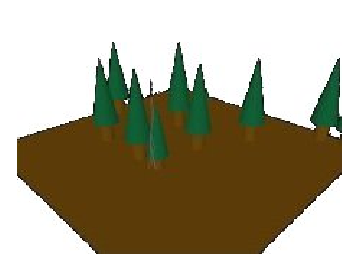
\includegraphics[width=3.5cm]{img/figura1.eps} &
		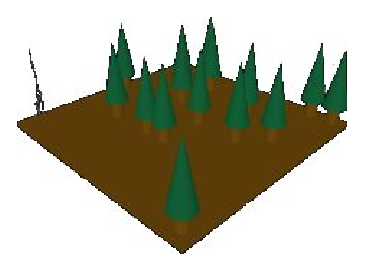
\includegraphics[width=3.5cm]{img/figura2.eps}
	\end{tabular}
 	\caption{\label{fig:ejemplo} Ejemplos de diferentes estados del tablero de juego}
\end{figure}

Se debe resaltar que no se est\'a interesado en el resultado propio del
modelo anterior, sino m\'as bien en definir un sistema de RV para este
modelo con el sistema propuesto en el cap\'itulo anterior.

Son cuatro los elementos principales que se deben definir. En primer
lugar se definir\'an los eventos necesarios para que el sistema pueda
ejecutar las actividades. En segundo lugar, se dise\~nar\'an los
generadores de eventos. En tercer lugar, se definir\'an los actores que
forman parte de la escena. Por \'ultimo, se introducir\'an las
primitivas que podr\'an hacer visible las diferentes partes que se
deseen mostrar.

Los eventos que se pueden producir en el sistema se muestran en la tabla \ref{table1}.


\begin{table}[h]
\begin{center}
\begin{small}
\begin{tabular}{|p{1cm}|p{2.6cm}|p{2.6cm}|}

	\hline
	\itshape Tipo de evento &
	\itshape Significado & 
	\itshape Datos asociados\\

	\hline
	$t$ & 
	Evento que se genera cada cierto tiempo $t$ & 
	Incremento del tiempo con respecto al anterior evento\\

	\hline
	$c$ &
	Crear un \'arbol en una determinada posici\'on &
	Posici\'on (i,j) donde se crea el \'arbol \\

	\hline
	$r$ &
	Creaci\'on de un rel\'ampago en una posici\'on &
	Posici\'on (i,j) donde se crea el rel\'ampago\\

	\hline
	$v$ &
	Elimina el \'arbol creado en una posici\'on &
	Posici\'on (i,j) donde se elimina el \'arbol\\

	\hline
	$q$ &
	Quemar un \'arbol en una posici\'on &
	Posici\'on (i,j) donde se quema el \'arbol\\

	\hline
	$d$ &
	Dibuja en OpenGL &
	Nada\\

	\hline

\end{tabular}
\end{small}
\caption{\label{table1} Definici\'on de eventos}
\end{center}
\end{table}



Los siguientes elementos que se deben definir son los generadores de
eventos. Estos son tres:

\[\begin{array}{c}
	G_{\mathit{tiempo}} = \{e^{t}\ \mathit{cada \ cierto \ tiempo \ t}\}\\

	G_{\mathit{bosque}} = \left\{
		\begin{matrix}
			e^{c} & \mathit{con \ probabilidad \ g}\\
			e^{r} & \mathit{con \ probabilidad \ f}
		\end{matrix}\right\}\\

	G_{\mathit{opengl}} = \{e^{d}\ \mathit{cada \ redibujado}\}
\end{array}\]

Por supuesto, podr\'iamos definir m\'as generadores. Por ejemplo, cuando pulsamos
un bot\'on se podr\'ia generar un evento $e^{r}$ y lanzar un rel\'ampago en la
posicion (i,j). Sin embargo, para este caso pr\'actico no es necesario.

En la table \ref{table2} se definen cada cada una de las primitivas y las
transformaciones.


\begin{table}[h]
\begin{center}
\begin{small}
\begin{tabular}{|l|l|}

	\hline
	\itshape Primitiva &
	\itshape Dibujo\\

	\hline
	$A$ &
	\'Arbol.\\

	\hline
	$A_{q}$ &
	\'Arbol quemado\\

	\hline
	$R$ &
	Rel\'ampago.\\

	\hline
	$B_{NxN}$ &
	Tablero de NxN que representa
	el bosque\\

	\hline
	\hline
	\itshape Transformaciones &
	\itshape Transformaci\'on\\

	\hline
	$T_{i,j}$ &
	Traslaci\'on $(i,j)$\\

	\hline
	$S_{s}$ &
	Escalado (s)\\
	
	\hline

\end{tabular}
\end{small}
\caption{\label{table2} Definici\'on de primitivas y transformaciones}
\end{center}
\end{table}


Las funciones $\gamma$, $I$, $F$ son implementadas para Opengl y dibujadas en una ventana.

Por \'ultimo, se especifican los actores que componen nuestro sistema. 
Para la definici\'on de un actor se debe definir la funci\'on de evoluci\'on
$\lambda$. La tabla \ref{table3} muestra los diferentes actores y su funci\'on de evoluci\'on.



\begin{table}[h]
\begin{center}
\begin{small}
\begin{tabular}{|p{0.6cm}|p{1.5cm}|p{4.1cm}|}

	\hline
	\itshape Actor &
	\itshape Descripci\'on &
	\itshape Funci\'on $\lambda$ \\

	\hline
	$B^{crv}$ &
	Representa el bosque &
	$\lambda (B^{crv}, e^{f})=\left\{
	\begin{matrix}
		AC^{t} \cdot B^{crv} & f = c \\
		R^{t} \cdot B^{crv} & f = r \\
		B^{crv} & f = v	\\
		B^{crv} & f \neq c, r, v
	\end{matrix}\right\}$ \\

	\hline
	$AC^{t}$ &
	Representa un \'arbol en crecimiento. &
	$\lambda (AC^{t}, e^{f}) = \left\{
	\begin{matrix}
		AC^{t+1}  &  f = t \\
		A^{q} & f = t \wedge t + 1 > N_{frames} \\
		AC^{t} & f \neq	t
	 \end{matrix}\right\}$ \\

	\hline
	$AR^{q}$ &
	\'Arbol &
	$\lambda (A^{q}, e^{f}) = \left\{
	\begin{matrix}
		AQ^{t}	& f = q \\
		A^{q} & f \neq q
	\end{matrix}\right\}$ \\
	
	\hline
	$R^{t}$ &
	Representa la animaci\'on de un rel\'ampago &
	$\lambda (R^{t}, e^{f}) = \left\{
	\begin{matrix}
		R^{t + 1} & f = t \\
		\Delta e^{q}  & f = t \wedge t + 1 > N_{frames} \\
		R^{t}  & f \neq t
	\end{matrix}\right\}$ \\

	\hline
	$AQ^{t}$ &
	\'Arbol quem\'andose &
	$\lambda (AQ^{t}, e^{f}) = \left\{
	\begin{matrix}
		AQ^{t + 1}  & f = t \\
		\Delta e^{v}  & f = t \wedge t + 1 > N_{frames} \\
		AQ^{t}  & f \neq t 
	\end{matrix}\right\}$ \\

	\hline

\end{tabular}
\end{small}
\caption{\label{table3} Descripci\'on de los actores}
\end{center}
\end{table}



Aclarar que en el caso del actor $B^{crv}$ y el del evento $e^{v}$, solo
cambiar\'a el estado interno del actor al asignar la posici\'on $(i,j)$
del evento como vac\'ia.

Ahora todos los actores deben tener una representaci\'on que se ver\'a
en el dispositivo visual. Para ello, se define la funci\'on
$\tau$ que se muestra en la tabla \ref{table4}.




\begin{table}[h]
\begin{center}
\begin{small}
\begin{tabular}{|l|l|}
	
	\hline
	\itshape Actor &
	\itshape Funci\'on ${\tau}$ \\

	\hline
	$B^{d}$ &
	$\tau (B^{d}(v),e^{f}) = \left\{
	\begin{matrix}
		B_{NxN}  &  f = d \\
		\epsilon & f \neq d
	\end{matrix}\right\}$	\\

	\hline
	$AC^{d}$ &
	$\tau (AC^{d}(v), e^{f}) = \left\{
	\begin{matrix}
		D_{(i,j)}(S_{s}(A))  &  f = d \\
		\epsilon  & f \neq d
	\end{matrix}\right\}$ 	\\

	\hline
	$A^{d}$ &
	$\tau (AR^{d}(v), e^{f}) = \left\{
	\begin{matrix}
		T_{(i,j)}(A)  &  f = d \\
		\epsilon  &  f \neq d
	\end{matrix}\right\}$ 	\\

	\hline
	$R^{d}$ &
	$\tau (R^{d}(v), e^{f}) = \left\{
	\begin{matrix}
		T_{(i,j)}(R)   &  f = d \\
		\epsilon  &  f \neq d
	\end{matrix}\right\}$	\\

	\hline
	$AQ^{d}$ &
	$\tau (AQ^{d}(v), e^{f}) = \left\{
	\begin{matrix}
		T_{(i,j)}(S_{s^{-1}}(A_{q}))   &   f = d \\
		\epsilon  &  f \neq d
	\end{matrix}\right\}$	\\

	\hline
\end{tabular}
\end{small}
\caption{\label{table4} Definici\'on de las funciones de dibujo}
\end{center}
\end{table}




Se debe aclarar que en el dibujado de AC, el escalado $S$ va a
corresponder a un escalado creciente dependiendo del estado actual del
actor, que ser\'a modificado dependiendo del evento
$e^{t}$. El efecto es el de un \'arbol que crece de menos
a m\'as. La escala para cada uno de los t vendr\'a definida por la
expresi\'on $s=\frac{t}{N}$, donde $N$ es el n\'umero de frames totales
de la animaci\'on.


En el caso de $AQ$, el escalado se va a aplicar en sentido inverso,
representado por $s^{-1}$. Esto significa que el
efecto es el de un \'arbol quem\'andose y menguando.

Por \'ultimo decir, que el dibujado de un rel\'ampago depender\'a del
instante $t$ en que se encuentre $R$, y que poco a poco se dibujar\'a un
rel\'ampago con un algoritmo dependiente de $t$.

Como se puede comprobar, en las animaciones el dibujo de los actores
siempre va a depender de $t$, que modificar\'a el estado del actor para
cambiar su representaci\'on seg\'un vaya desarroll\'andose la
animaci\'on.

Para terminar se debe definir la cadena inicial:
$w_{0} = B^{\mathit{crv}}$

Con esta \'ultima expresi\'on queda terminada la definici\'on de todos
los elementos que componen el sistema de RV para modelar una
simulaci\'on de incendios forestales producido por rel\'ampagos. Para
ver como funciona el algoritmo propuesto en el cap\'itulo anterior, se
va a suponer que los generadores definidos anteriormente construyen
varios eventos. Dada la cadena inicial, el sistema evolucionar\'ia de
la siguiente manera:

\begin{itshape}
	Paso 3. $e^{*} = E(G^{*}, t) = \{ e^{t}, e^{c}, c^{d}\} = \{ e^{tcd}\}$
	
	Paso 4. $e^{v} = e^{d}$
	
	Paso 5. $e^{u} = e^{*} - e^{v} = e^{ct}$
	
	Paso 6. $w_{sig} = \alpha(w, e^{ct}) = \lambda(B^{crv}, e^{ct}) = AC^{0} \cdotp B^{crv}$
	
	Paso 7. $v = \Omega(w, e^{v}) = \Omega(B^{crv}, e^{d}) = \tau(B^{cr}, e^{d}) = B_{NxN}$
	
	Paso 8. $\Phi(v) = \Phi(B_{NxN}) = \gamma(B_{NxN})$
	
	Paso 9. $w = w_{sig}$ \ \ y \ \ $t = t + 1$
	
	Paso 11. Ir a paso 3
	
	Paso 3. $e^{*} = E(G^{*}, t) = \{ e^{t}, e^{r}, c^{d}\} = \{e^{trd}\}$
	
	Paso 4. $e^{v} = e^{d}$
	
	Paso 5. $e^{u} = e^{*} - e^{v} = e^{rt}$
	
	{Paso 6. \raggedright $w_{sig} = \alpha(AC^{0} \cdotp B^{crv}, e^{rt}) =$ \\
	\ \ \ \ \ \ $= \lambda(AC^{0}, e^{t}) \cdotp \lambda(B^{crv}, e^{r}) = AC^{1} \cdotp R^{0} \cdotp B^{crv}$}
	
	{Paso 7. \raggedright  $v = \Omega(AC^{0} \cdotp B^{crv}, e^{v}) =$ \\ 
	\ \ \ \ \ \ $= \tau(AC^{0}, e^{d}) \cdotp \tau(B^{cr}, e^{d}) = T_{(i,j)}(S_{0}(A)) \cdotp B_{NxN}$}
	
	
	{Paso 8. \raggedright $\Phi(D_{(i,j)}(S_{0}(A)) \cdotp T) = $\\
	\ \ \ \ \ \ $= I(T_{(i,j)}) \cdotp I( S_{0} ) \cdotp \gamma(A) \cdotp F(S_{0}) \cdotp F(T_{(i,j)}) \cdotp \gamma(B_{NxN})$}
	
	
	Paso 9. $w = w_{sig}$ y $t = t + 1$


   	Paso 11. Ir a paso 3


   	.....
\end{itshape}




%___________________________________________________________________________
\section{Conclusiones y trabajos futuros
\label{sec:conclusiones}}
%___________________________________________________________________________

Se ha presentado un modelo con un objetivo prioritario, la separaci\'on de la actividad de 
un sistema gr\'afico de la de los dispositivos visuales y de interacci\'on 
que componen dicho sistema.

Por uno lado, se tiene un lenguaje definido mediante gram\'aticas
independientes del contexto que detalla los elementos que componen el
sistema. Se establecen determinadas funciones que representan la
evoluci\'on de cada uno de los elementos a trav\'es del tiempo. Se
definen funciones que extraen la representaci\'on gr\'afica de los
elementos. Esta representaci\'on se env\'ia a los dispositivos visuales
mediante funciones que separan la implementaci\'on concreta sobre un
dispositivo visual y la descripci\'on gr\'afica del elemento,
eliminando la dependencia del sistema de los dispositivos gr\'aficos.

La separaci\'on de los dispositivos de entrada de la
definici\'on del sistema se ha articulado a trav\'es de los generadores
de eventos, que levantan una capa entre el hardware de entrada y la
representaci\'on del sistema. Para enlazar las acciones generadas por
los dispositivos de entrada se utiliza el modelo de eventos.

En general, se puede comprobar que todo el modelo intenta separar las
partes dependientes del tipo de dispositivo de las de la definici\'on
formal de un sistema de RV. La t\'ecnica empleada para dicha
separaci\'on es utilizar modelos matem\'aticos que transformen las
acciones de los dispositivos, tanto visuales como de entrada, en
acciones m\'as generales que puedan ser identificados por el sistema
independientemente del origen de la acci\'on, mediante abstracciones.

Esto supone varias ventajas: en primer lugar los dispositivos de entrada pueden 
ser sustituidos por otros dispositivos o por simulaciones de estos. Por otro lado existe 
la posibilidad de que los elementos del sistema sean reutilizados. Adem\'as, la representaci\'on 
de los elementos puede ser visual o no visual, e incluso ser diferente 
dependiendo del dispositivo de visualizaci\'on o 
de las necesidades del usuario. As\'i, si el dispositivo tiene unas caracter\'isticas 
concretas, la representaci\'on siempre se podr\'a adaptar al dispositivo. Por \'ultimo, varios 
actores pueden relacionarse entre s\'i envi\'andose mutuamente eventos que ambos reconozcan.

Con el sistema planteado se puede dise\~nar f\'acilmente un motor f\'isico utilizando los 
elementos de la escena. Esto se realiza dise\~nando generadores de eventos de diferentes 
tipos, dependiendo de la caracter\'istica f\'isica y activando la actividad del actor 
necesaria para que este reaccione ante el proceso f\'isico. Por ejemplo, si se quiere 
que un actor reaccione ante una colisi\'on, el generador de eventos de este tipo calcular\'a 
las colisiones de los elementos extrayendo la geometr\'ia de la escena gracias al motor 
gr\'afico (utilizando la implementaci\'on de las funciones $\gamma$, I, F para calcular los cubos 
envolventes de los elementos) y generando los eventos necesarios para las colisiones. Si 
el sistema lo permite, se podr\'ia implementar mediante hardware este generador de eventos.

El motor de IA puede ser dise\~nado en las funciones de evoluci\'on de los actores. En estas funciones es donde cada actor va a tomar sus decisiones dependiendo de su estado actual. Mediante eventos se pueden ejecutar actividades que cambien el estado del actor y que modifiquen su comportamiento. Adem\'as, como el propio actor puede generar eventos es posible dise\~nar procesos de retroalimentaci\'on utilizados en IA. Adem\'as la integraci\'on entre motor f\'isico y motor de IA est\'a garantizada ya estos dos motores se relacionan entre s\'i mediante los eventos.

El uso de un lenguaje para la descripci\'on de los elementos de la escena y la independencia del sistema gr\'afico hace que estas cadenas descriptivas puedan ser utilizadas en cualquier otro sistema, siempre y cuando est\'an implementados los elementos b\'asicos (todas las funciones sem\'anticas explicadas).

El modelo presentado en este trabajo est\'a actualmente en desarrollo y se desea
seguir desarrollando los diferentes aspectos tratados aqu\'i. Uno de los puntos a 
investigar y que se apuntan en el art\'iculo es la optimizaci\'on del algoritmo
y su paralelizaci\'on. La definici\'on del sistema mediante cadenas facilita
la posibilidad de algoritmos paralelos. Por otro lado, las cadenas representan
estados del sistema y su evoluci\'on. Esta evoluci\'on puede variar mediante 
mutaciones y se puede investigar posibles soluciones evolutivas para el dise\~no del sistema.
Por otro lado, se puede estudiar la posibilidad de activar eventos con una cierta
probabilidad. Es decir, un actor activar\'ia una actividad, ya no solo cuando
suceda un determinado evento, sino que este se activase con una cierta probabilidad.
As\'i un actor podr\'ia definirse como $a^{p(e^{1}),p(e^{2})}(w)$, siendo $p(e^{i})$ la probabilidad
de reaccionar al evento $e^{i}$.

En definitiva, se ha pretendido dise\~nar un sistema reutilizable, gen\'erico y que se pueda incrementar 
y adaptar f\'acilmente, en el que la parte fundamental, que es la evoluci\'on en el tiempo, sea independiente 
de c\'omo se represente y con qui\'en interact\'ue.




%___________________________________________________________________________
% ---- Bibliography ----
%___________________________________________________________________________

\bibliographystyle{eg-alpha}
%\bibliography{gabriel_lg}


\begin{thebibliography}{\uppercase{JHM07}}

\bibitem[PhyX]{Physx}
\textsc{PhysX by AGEIA}:
\httpAddr{//physx.ageia.com/}

\bibitem[DJK05]{David2005}
\textsc{David J.~Kasik William~Buxton D. R.~F.}:
\newblock Ten cad challenges.
\newblock \emph{IEEE Computer Graphics and Applications 25} (2005), 81--90.

\bibitem[WMod]{WModel}
\textsc{Working Model: Simulaci\'on de Sistemas}:
\httpAddr{//www.design-simulation.com}

\bibitem[DW94]{Davis1994}
\textsc{Davis Martin D.;~Sigal R., Weyuker E.~J.}:
\newblock \emph{Computability, Complexity, and Languages, Fundamentals of
  Theoretical Computer Science}, 2nd~ed.
\newblock San Diego: Elsevier Science, 1994.

\bibitem[NGDy]{NGDynamics}
\textsc{Newton Game Dynamics}:
\httpAddr{//www.newtondynamics.com/}

\bibitem[ODEn]{ODE}
\textsc{Open Dynamics Engine}:
\httpAddr{www.ode.org}

\bibitem[WPEn]{Wikipedia2007}
\textsc{Wikipedia - Physics engine}:
\httpAddr{//en.wikipedia.org/wiki/physics_engine}

\bibitem[Havok]{Havok}
\textsc{Havok}:
\httpAddr{//www.havok.com/}

\bibitem[JHM07]{John2007}
\textsc{John H.~Miller S. E.~P.}:
\newblock \emph{Complex Adaptative Systems}.
\newblock Princeton University Press, 2007.

\bibitem[JS04]{Joshua2004}
\textsc{Joshua~Strickon J. A.~P.}:
\newblock Emerging technologies.
\newblock \emph{Siggraph} (2004).

\bibitem[PALay]{PAL}
\textsc{PAL: Physics Abstraction Layer}:
\httpAddr{//www.adrianboeing.com/pal/}

\bibitem[DirX]{DirectX}
\textsc{P\'agina oficial de DirectX}:
\httpAddr{//www.microsoft.com/windows/directx/default.mspx}

\bibitem[OpGL]{OpenGL}
\textsc{P\'agina oficial de OpenGL}:
\httpAddr{//www.opengl.org/}

\bibitem[SDLay]{SDL}
\textsc{Simple DirectMedia Layer (SDL)}:
\httpAddr{//www.libsdl.org/}

\bibitem[OGRE]{OGRE}
\textsc{OGRE 3D : Open source graphics engine}:
\httpAddr{//www.ogre3d.org/}

\bibitem[VTK]{VTK}
\textsc{The Visualization ToolKit (VTK)}:
\httpAddr{//public.kitware.com/vtk/}

\bibitem[EOECF]{EOECF}
\textsc{EO Evolutionary Computation Framework}:
\httpAddr{//eodev.sourceforge.net/}

\bibitem[CILib]{CILib}
\textsc{CILib (Computational Intelligence Library)}:
\httpAddr{//cilib.sourceforge.net/}

\bibitem[Jade]{Jade}
\textsc{Jade - Java Agent DEvelopment Framework}:
\httpAddr{//jade.tilab.com/}

\bibitem[Lai01]{Laird2001}
\textsc{Laird J.~E.}:
\newblock Using a computer game to develop advanced ai.
\newblock \emph{Computer 34 (7)} (2001), 70--75.

\bibitem[GNY04]{Georgios2004}
\textsc{Georgios N.~Yannakakis John~Levine J.~H.}:
\newblock An evolutionary approach for interactive computer games.
\newblock \emph{In Proceedings of the Congress on Evolutionary Computation}
  (2004), 986--993.

\bibitem[CM07]{Chris2007}
\textsc{Chris~Miles Juan~Quiroz R. L. S. J.~L.}:
\newblock Co-evolving influence map tree based strategy game players.
\newblock \emph{IEEE Symposium on Computational Intelligence and Games} (2007),
  88--95.

\bibitem[RGR05]{Robert2005}
\textsc{Robert G.~Reynolds Ziad~Kobti T. A. K. L. Y. L.~Y.}:
\newblock Unraveling ancient mysteries: Reimagining the past using evolutionary
  computation in a complex gaming environment.
\newblock \emph{IEEE transactions on evolutionary computation 9} (2005),
  707--720.

\bibitem[Woo97]{Wooldridge1997}
\textsc{Wooldridge M.}:
\newblock Agent-based software engineering.
\newblock \emph{IEEE Proceedings Software Engineering 144} (1997), 26--37.

\bibitem[WD00]{Wood2000}
\textsc{Wood M.~F., DeLoach S.}:
\newblock An overview of the multiagent systems engineering methodology.
\newblock \emph{AOSE} (2000), 207--222.

\bibitem[Ken06]{Kenyon2006}
\textsc{Kenyon S.~H.}:
\newblock Behavioral software agents for real-time games.
\newblock \emph{IEEE Potentials 25} (2006), 19--25.

\bibitem[AK02]{Aaron2002}
\textsc{Aaron~Khoo R.~Z.}:
\newblock Applying inexpensive ai techniques to computer games.
\newblock \emph{IEEE Intelligent Systems 17(4)} (2002), 48--53.

\end{thebibliography}




\end{document}
